\documentclass[a4paper,12pt]{report}

\usepackage{alltt, fancyvrb, url}
\usepackage{graphicx}
\usepackage{subfigure}
\usepackage{array}
\usepackage{wrapfig}
\usepackage{algorithmic}
\usepackage[utf8]{inputenc}
\usepackage{fontenc}
\usepackage{amsmath,stmaryrd,mathtools,algorithm}
\usepackage{amssymb}
\usepackage{float}
\usepackage{hyperref}

\begin{document}

    
	\title{Elaborato per il corso di Basi di dati}
	\author{Davide Carità - 0000873616}
	\date{}
	
    \maketitle
	\tableofcontents*
	\newpage


	\addcontentsline{toc}{chapter}{Analisi dei requisiti} 
	\chapter*{Analisi dei requisiti}
    Si vuole realizzare una base di dati che supporti le funzionalità di 
    un'applicazione di compravendita di immobili nonché il monitoraggio del 
    welfare delle principali città europee. Uno dei servizi sarà quello di 
    filtrare le città in base alle proprie esigenze: si potrà vedere ad 
    esempio quale città ha ottenuto i migliori punteggi a livello europeo 
    in tema di qualità dell'aria, costo della vita o efficienza sanitaria. 
    Una volta trovata la propria città ideale, verranno visualizzati vari 
    annunci immobiliari suddivisi per zone della città. All'interno 
    dell'annuncio, verranno mostrati i dettagli relativi all'immobile: 
    metratura, numero stanze, prezzo, etc\dots
    Inoltre, il servizio fornirà la funzionalità di avviare una conversazione tra 
    acquirente e venditore, offrendo loro la possibilità di scambiarsi
    informazioni in modo rapido.

    Sarà offerta ai giudici d'esecuzione l'opportunità di creare un utente 
    che avrà il privilegio di gestire aste immobiliari

    	\addcontentsline{toc}{section}{Requisiti in linguaggio naturale} 
        \section*{Requisiti in linguaggio naturale}
    	






    	\addcontentsline{toc}{section}{Estrazione dei concetti principali} 
    	\section*{Estrazione dei concetti principali}
            A seguito della lettura e comprensione dei requisiti richiesti dal cliente, si procede sviluppando un testo che
            ne riassuma tutti i concetti e in particolare ne estragga quelli principali, risultando essere in questo modo
            meglio fruibile per la realizzazione della base di dati.
            
            \begin{center}
                 \begin{tabular}{|c c c|} 
                     \hline
                     Termine & Breve descrizione & Sinonimi \\ [0.5ex] 
                     \hline
                \end{tabular}
            \end{center}
            
            Di seguito le azioni che sono richieste:
            
            \begin{enumerate}
              \item a
              \item b
              \item c
              \item d
              
            \end{enumerate}


	\chapter{Progettazione concettuale}
        La progettazione concettuale, derivata dall'analisi dei concetti principali del dominio,
        è stata incrementale in termini di complessità. Di seguito passeremo quindi in rassegna
        gli stadi dello schema cronologicamente ordinati, illustrando le motivazioni che hanno 
        portato ad effettuare i vari raffinamenti. 

        \section{Schema scheletro}
        Il primo schema è il risultato della trasposizione su E/R delle astrazioni formulate nel capitolo precedente.
        In primo piano figura l'entita \textit{città}, caratterizzata da al più N \textit{valutazioni} generiche,
        ciascuna delle quali espressa con un punteggio intero nell'intervallo [0,10]. \\
        \\
        La città è identificata da un codice univoco, in modo da evitare di incappare in uno dei ricorrenti scenari di 
        città omonime nella medesima nazione (dove lo stato ed il nome della città non sarebbero sufficienti a distinguerle). Sebbene in molti casi ciò possa essere risolto specificando la regione di appartenenza 
        delle città "doppione", rimarrebbero comunque insolute casistiche tipiche del territorio britannico, dove città omonime 
        potrebbero situarsi in contee diverse ma all'interno della stessa "Government Office \textit{Region}". A titolo di esempio, basti
        pensare che nell'intero UK compaiono 14 città chiamate Newport! \footnote{https://www.southwalesargus.co.uk/news/19433701.newports-across-world/} \\
        \\
        Un annuncio riguarda un solo immobile, mentre lo stesso immobile può comparire in più annunci diversi. Quest'ultima cardinalità,
        meno ovvia, deriva dall'esigenza di conservare lo storico di tutte le vendite/affitti di ciascuna abitazione, in modo da formulare
        in seguito un trend del prezzo in funzione del tempo (da presentare agli interessati).

        \begin{figure}[ht]
            \centering{}
            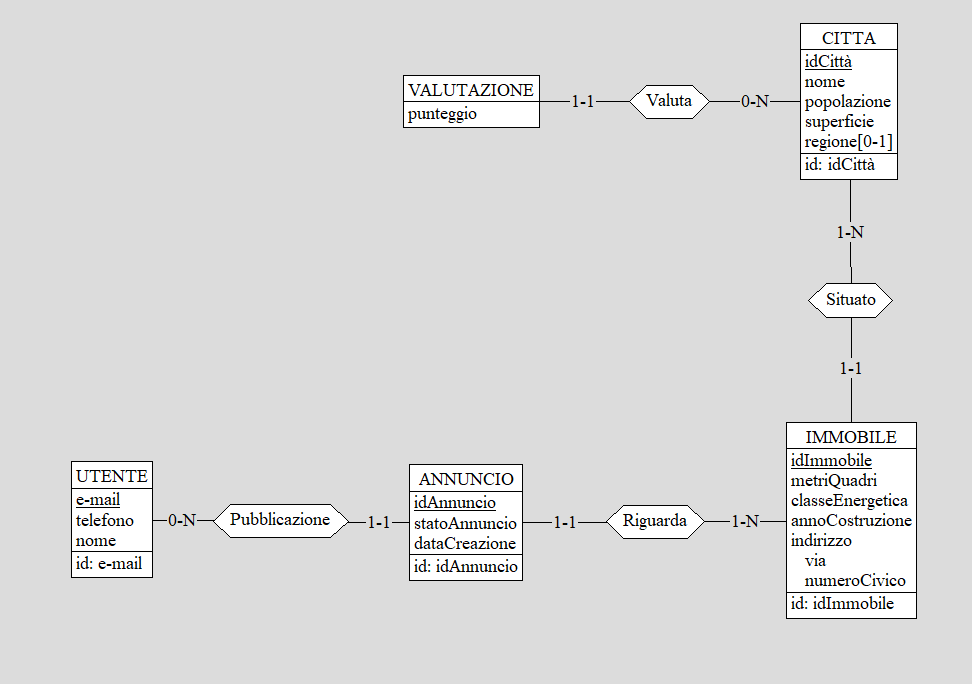
\includegraphics[width=\linewidth]{./images/first.png}
            \caption{La prima versione dello schema concettuale}
        \end{figure}

        \section{Divisione in zone e di immobili}
        
        ...

        Introducendo una gerarchia per differenziare le varie tipologie di \textit{immobili} inserite negli annunci,
        ogni immobile dovrà essere necessariamente contraddistinto da un ID proprio. Perchè? Se tutte le dimore
        fossero case indipendenti, allora potrebbero essere identificate da attributi che ne specifichino la posizione.
        Aggiungendo gli appartamenti poi, basterebbe includere nella chiave un campo che indichi il numero dell'interno.
        Con l'avvento delle stanze singole tuttavia, la soluzione precedentemente adottata risulterà inadatta, poichè 
        non risponderebbe alla necessità di un utente di affittare più stanze della stessa abitazione (ognuna con un 
        annuncio dedicato).

        \begin{figure}[ht]
            \centering{}
            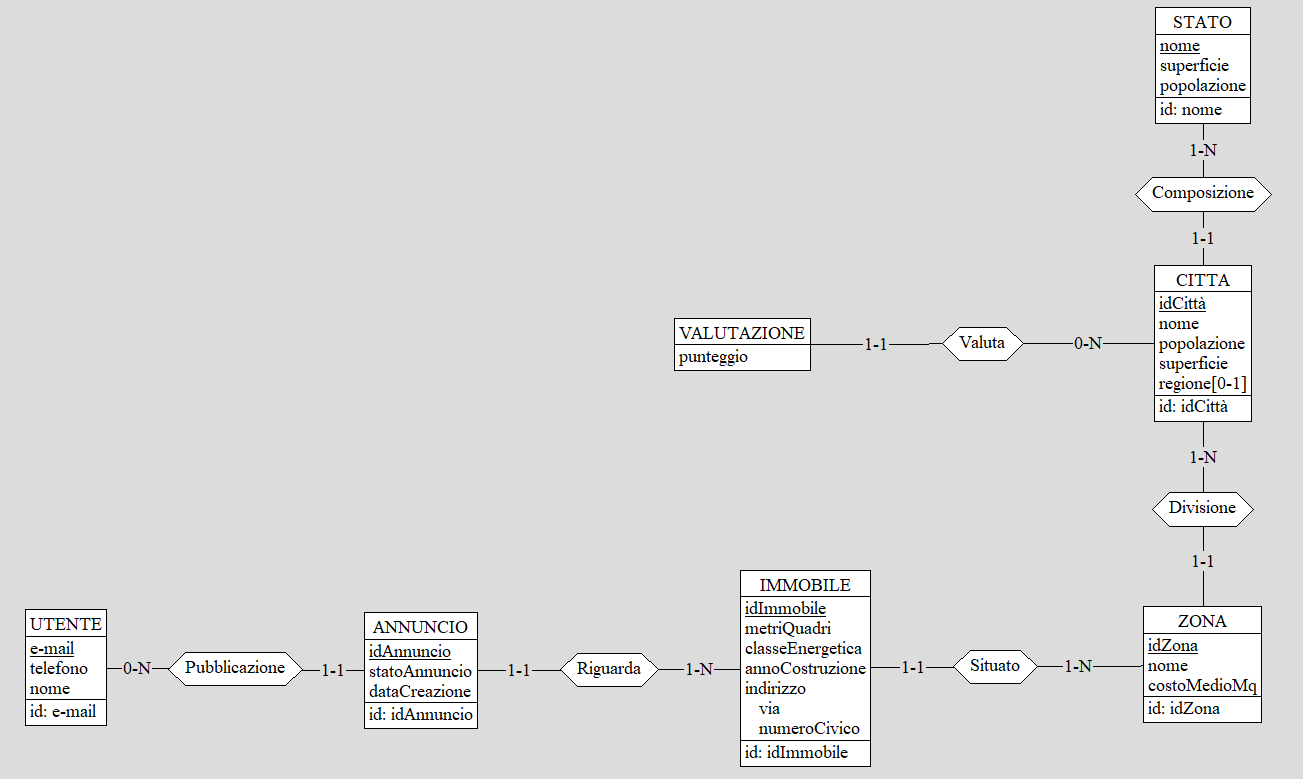
\includegraphics[width=\linewidth]{./images/second.png}
            \caption{La seconda versione dello schema concettuale}
        \end{figure}

        \section{Espansione delle valutazioni}
        Nell’amplificazione della porzione di schema relativa all’analisi delle città abbiamo scisso la precedente entità 
        “segnaposto” \textit{valutazione} in una serie di categorie, come illustrato nei requisiti. Ciascuna di queste è caratterizzata 
        da parametri dal dominio numerico (e.g. \textit{ambiente} da \textit{PM2.5media} e \textit{percentualeSpazioVerdeUrbano}), in
        base ai cui valori verrà calcolato in automatico un punteggio onnicomprensivo per la categoria, poi conservato nel campo 
        corrispondente di \textit{città\textunderscore anno} (\textit{punteggioAmbiente} nell’esempio citato). \\
        \\
        Il ruolo dell’entità \textit{città\_anno} è quello di consentire la storicizzazione dei punteggi ottenuti da ciascuna città 
        negli anni passati, in modo da poter computare lo sviluppo, o l’involuzione, a cui il luogo ha assistito. Ciascuna istanza 
        di categoria può far riferimento a più città ed in più anni diversi: Parigi e Londra potrebbero aver registrato stessi 
        \textit{PILProCapite, stipendioMedio e tassoDisoccupazione} nel 2019, così come Heidelberg potrebbe aver riconfermato gli 
        stessi valori relativi alla \textit{sanità} dell'anno precedente. Ad ogni \textit{città\_anno}, invece, è collegata una ed 
        una sola istanza di tutte le 5 categorie. \\
        \\
        
        \begin{figure}[ht]
            \centering{}
            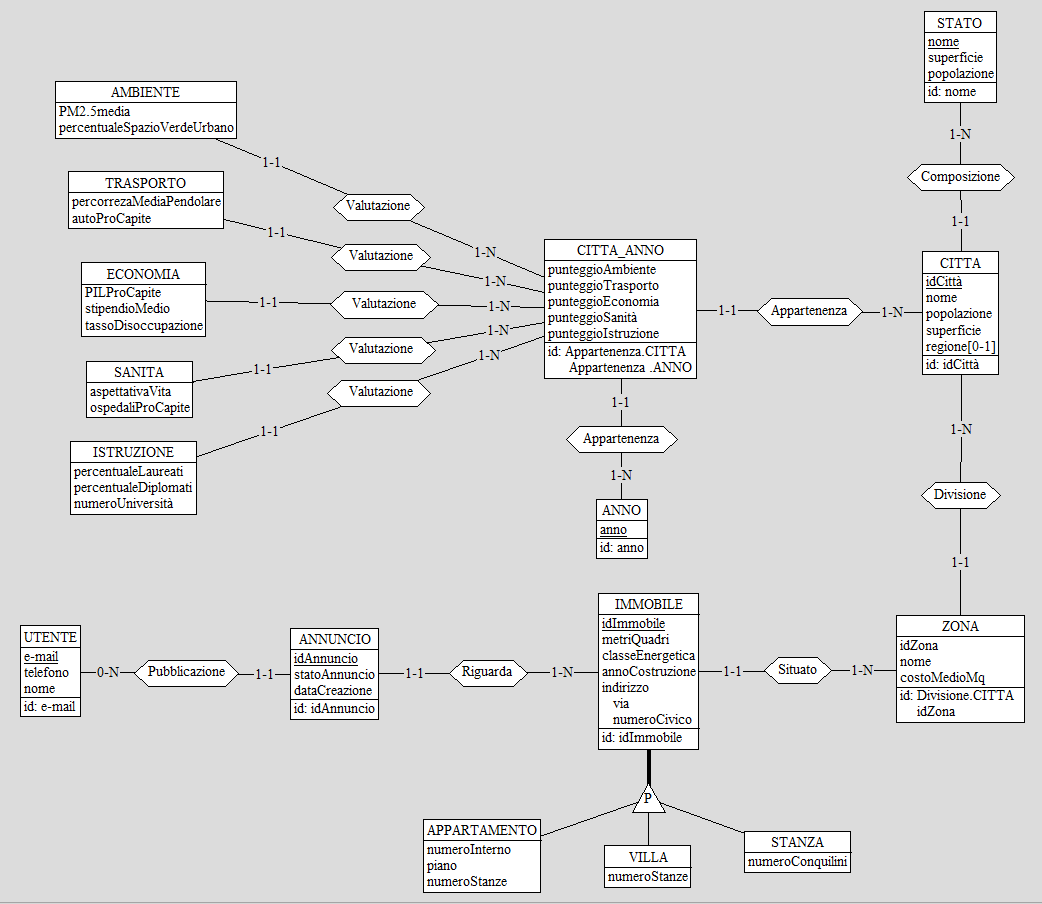
\includegraphics[width=\linewidth]{./images/third.png}
            \caption{La terza versione dello schema concettuale}
        \end{figure}
        	
    	\section{Schema finale}
        La messaggistica viene modellata attraverso le associazioni tra le entità \textit{utente $\Leftrightarrow$ messaggio} e 
        \textit{messaggio $\Leftrightarrow$ annuncio\_utente}. In prima battuta ci si potrebbe erroneamente domandare il motivo 
        del non aver optato per una relazione ad anello tra \textit{utenti}, con il testo del messaggio racchiuso in un campo 
        dell’ associazione, tuttavia tale configurazione consentirebbe di memorizzare nella base di dati al più un 
        \textit{messaggio} per ogni coppia di utenti! \\
        \\
        Sarebbe inoltre fuorviante collegare ogni messaggio direttamente 
        a mittente e destinatario poiché non si terrebbe conto del caso in cui le stesse due persone dovessero contattarsi in merito ad annunci 
        diversi, anche contemporaneamente, e non si riuscirebbe dunque a dedurre il contesto dei messaggi. Per risolvere quest’ultima problematica 
        si è deciso di interporre l'enitità \textit{messaggio} tra \textit{utente}, nonchè il potenziale acquirente, ed \textit{annuncio\_utente}, 
        ossia il gestore dell’inserzione nelle vesti del suo annuncio. I messaggi all’interno di ogni chat vengono identificati dall’istante 
        temporale in cui sono inviati (timestamp).



        \begin{figure}[ht]
            \centering{}
            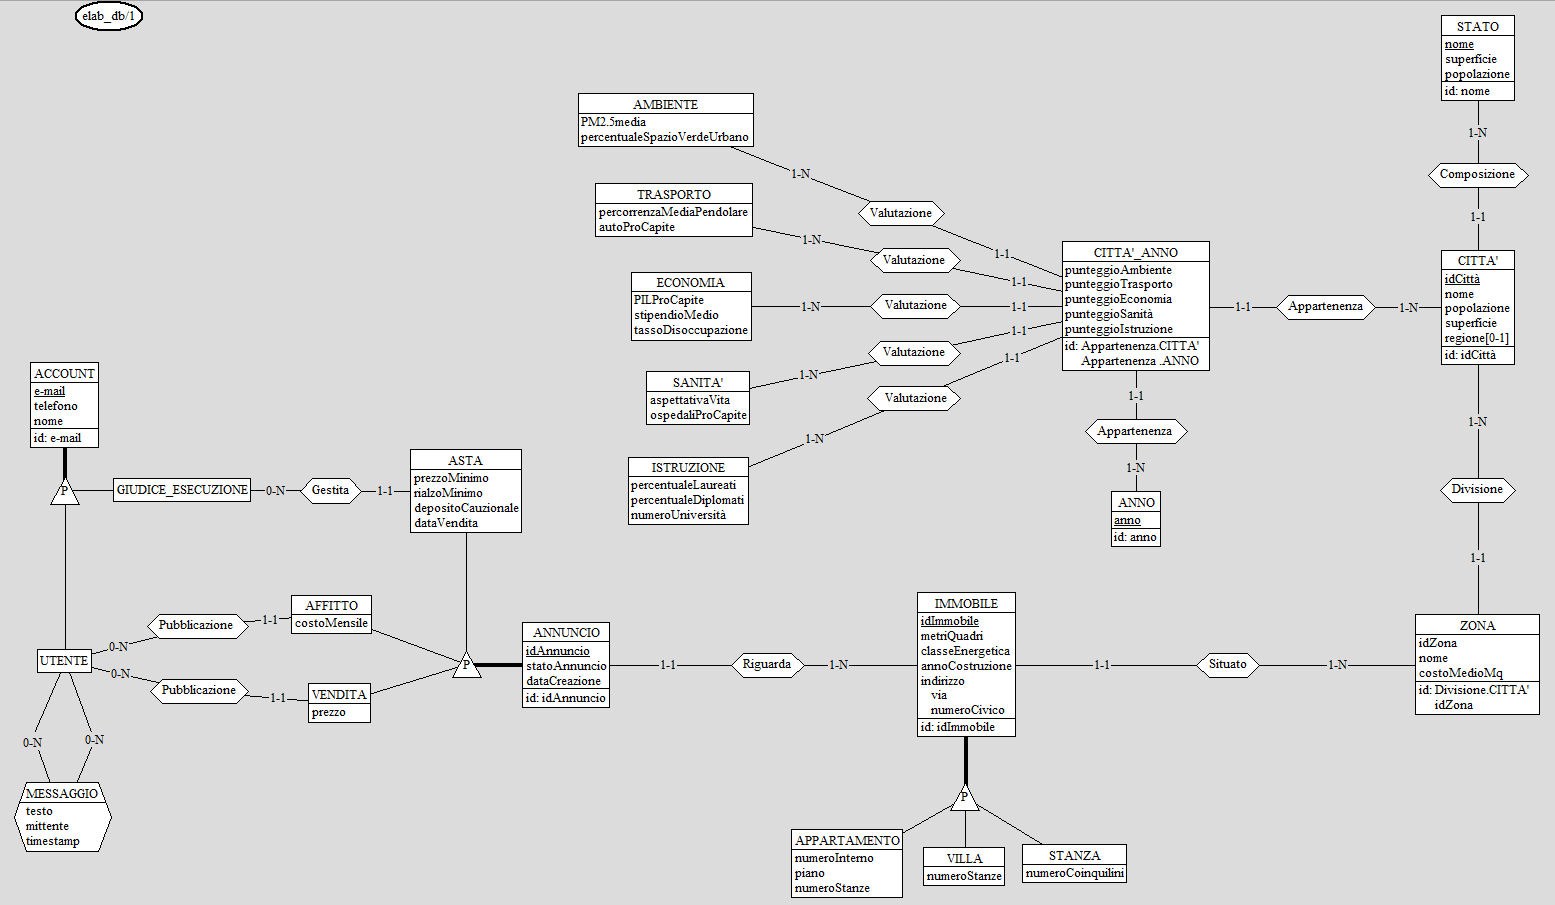
\includegraphics[width=\linewidth]{./images/fourth.png}
            \caption{L'ultima versione dello schema concettuale}
        \end{figure}

        	
    \addcontentsline{toc}{chapter}{Progettazione logica}
	\chapter*{Progettazione logica}
    	\addcontentsline{toc}{section}{Stima del volume dei dati} 
    	\section*{Stima del volume dei dati}
        	asdasd
         	
        \addcontentsline{toc}{section}{Descrizione delle operazioni principali e stima della loro frequenza} 
    	\section*{Descrizione delle operazioni principali e stima della loro frequenza}
        	asdasd
        	
        \addcontentsline{toc}{section}{Schemi di navigazione e tabelle degli accessi} 
    	\section*{Schemi di navigazione e tabelle degli accessi}
        	asdasd
        	
        \addcontentsline{toc}{section}{Analisi delle ridondanze} 
    	\section*{Analisi delle ridondanze}
        	asdasd
        	
        \addcontentsline{toc}{section}{Traduzione di entità e associazioni in relazioni} 
    	\section*{Traduzione di entità e associazioni in relazioni}
        	asdasd
        	
        \addcontentsline{toc}{section}{Schema relazionale finale} 
    	\section*{Schema relazionale finale}
        	asdasd
        	
        \addcontentsline{toc}{section}{Descrizione dell'architettura dell'applicazione realizzata} 
    	\section*{Descrizione dell'architettura dell'applicazione realizzata}
        	asdasd
        	

    \addcontentsline{toc}{chapter}{Progettazione dell'applicazione}
	\chapter*{Progettazione dell'applicazione}
	
    	\addcontentsline{toc}{section}{Traduzione delle operazioni in query SQL} 
    	\section*{Traduzione delle operazioni in query SQL}
    	    asdasd
 
\end{document}